\documentclass[11pt,a4paper]{article}

% MSX StepUp HybridHLE user manual (English edition).
% Build both editions from this directory with: make
\usepackage[utf8]{inputenc}
\usepackage[T1]{fontenc}
\usepackage[english]{babel}
\usepackage[a4paper,margin=22mm,headheight=15pt]{geometry}
\usepackage{graphicx}
\usepackage{array}
\usepackage{tabularx}
\usepackage{booktabs}
\usepackage{xcolor}
\usepackage{hyperref}
\usepackage{fancyhdr}
\usepackage{enumitem}

\definecolor{msxblue}{HTML}{087EB8}
\definecolor{stepred}{HTML}{EF3B45}
\definecolor{ink}{HTML}{172033}
\definecolor{softblue}{HTML}{EAF6FB}
\definecolor{softgray}{HTML}{F2F4F7}

\hypersetup{
  colorlinks=true,
  linkcolor=msxblue,
  urlcolor=msxblue,
  pdftitle={MSX StepUp HybridHLE User Manual},
  pdfauthor={DiHalt (Fernando García and Clemente Tiñena)}
}

\graphicspath{{../../assets/graphics/}}
\setlength{\parindent}{0pt}
\setlength{\parskip}{0.65em}
\setlist{itemsep=0.25em,topsep=0.35em}
\renewcommand{\arraystretch}{1.25}

\pagestyle{fancy}
\fancyhf{}
\fancyhead[L]{\textcolor{msxblue}{MSX StepUp HybridHLE}}
\fancyhead[R]{User Manual}
\fancyfoot[C]{\thepage}
\renewcommand{\headrulewidth}{0.4pt}

\newcommand{\keycap}[1]{%
  \begingroup
  \setlength{\fboxsep}{3pt}%
  \colorbox{softgray}{\texttt{#1}}%
  \endgroup
}

\newcommand{\noticebox}[2]{%
  \begin{center}
  \fcolorbox{#1}{softblue}{%
    \begin{minipage}{0.91\textwidth}
      #2
    \end{minipage}}
  \end{center}
}

\begin{document}

\begin{titlepage}
  \thispagestyle{empty}
  \centering
  \vspace*{8mm}
  
\includegraphics[width=0.76\textwidth]{stepup_logo.png}

  \vspace{8mm}
  {\Huge\bfseries\color{ink} User Manual\par}
  \vspace{2mm}
  {\Large The original MSX game, wrapped in a modern layer\par}

  \vfill
  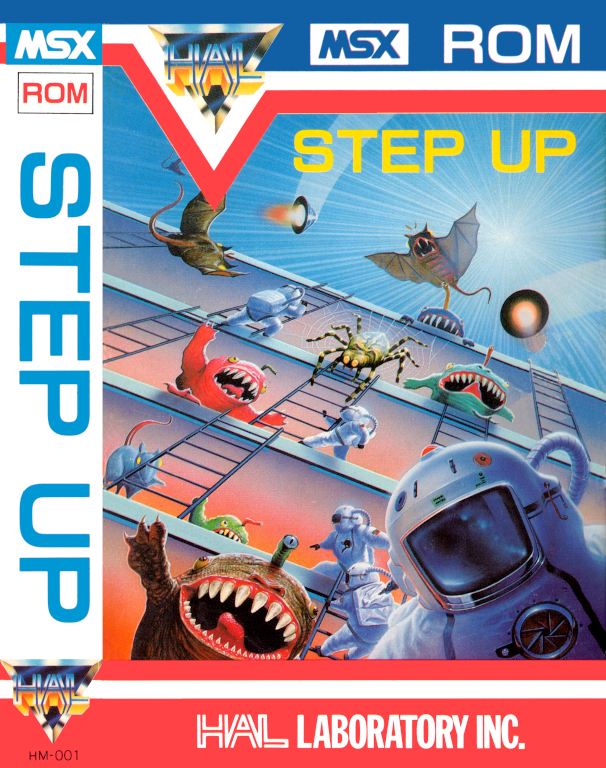
\includegraphics[height=0.59\textheight,keepaspectratio]{intro.png}
  \vfill

  {\large Version 1.0 --- August 2026\par}
  \vspace{2mm}
  {\small DiHalt --- Fernando García and Clemente Tiñena\par}
\end{titlepage}

\tableofcontents
\newpage

\section{Welcome to Step Up}

\textit{Step Up} is an action platform game originally released for MSX in
1983 and developed by Takara and Marvel Soft. You play a lone astronaut
stranded on a hostile planet. His only chance of returning home is to climb to
the rooftop and reach the waiting spaceship.

\textbf{MSX StepUp HybridHLE preserves the original cartridge program.} This
is not a remake that imitates its rules: the original Z80 instructions still
decide movement, collisions, enemies, scoring, lives, and progression between
stages. Godot acts as a modern outer layer that runs and presents that program
on Windows, Linux, macOS, and Android.

\noticebox{stepred}{\textbf{Important.} The original cartridge is not
distributed with this project. To play, you need a legally obtained dump of
your own \textit{Step Up} cartridge.}

\section{Getting started}

\subsection{First launch}

\begin{enumerate}
  \item Open \textbf{MSX StepUp HybridHLE}.
  \item When the setup screen appears, select
        \textbf{Select Step Up ROM}.
  \item Choose your cartridge's \texttt{.rom} file. If it is inside a ZIP
        archive, extract it first.
  \item The application accepts 8, 16, or 32 KiB dumps, extracts the valid
        8 KiB bank, and stores a private copy for future launches.
\end{enumerate}

On desktop computers, you may instead create a \texttt{roms} directory beside
the executable and save the file as \texttt{roms/stepup.rom}. On macOS, place
the directory beside the \texttt{.app} bundle, not inside it.

\subsection{Starting a game}

An opening illustration is displayed for a few seconds after the game loads.
Press \keycap{Space} ---or \textbf{ACTION} on Android--- to skip it. On the
title screen, use the action button again to start when prompted by the game.

\section{Game objective}

The building has ten floors, marked F1 through F10 and connected by blue
ladders. Guide the astronaut from the lower area to the rooftop while avoiding
the creatures and moving hazards patrolling each floor.

Once you reach the roof, a small spaceship appears. \textbf{Reaching the top
is not enough: you must jump aboard before it flies away.} Succeed and you
advance to the next stage; wait too long and you will be left exposed to the
enemies on the rooftop.

\subsection{Hazards}

Each threat behaves differently. You will encounter:

\begin{itemize}
  \item mice or rats that scurry along the platforms;
  \item bats that fly vertically;
  \item monsters that move along ladders and floors;
  \item spiders that periodically emerge from their webs;
  \item moving obstacles such as the red girder.
\end{itemize}

Contact can knock the astronaut to the ground and costs one life. After losing
a life, you start again from the bottom. A game begins with three lives, and
an extra life is awarded every 10,000 points.

\subsection{Energy barrier}

The astronaut has temporary protection. While it is active, the character
turns red and consumes part of the energy gauge at the bottom of the screen.
The supply is restored at the beginning of every new life or stage; if it runs
out, the character is defeated.

Later stages retain the same objective but increase the pressure and the
number of hazards; for example, more spider webs appear.

\section{Controls}

\begin{center}
\begin{tabularx}{\textwidth}{>{\bfseries}p{0.28\textwidth}XX}
\toprule
Action & Desktop & Android \\
\midrule
Walk left or right & \keycap{$\leftarrow$} / \keycap{$\rightarrow$} & LEFT / RIGHT \\
Climb up or down & \keycap{$\uparrow$} / \keycap{$\downarrow$} & UP / DOWN \\
Jump or perform an action & \keycap{Space} & ACTION \\
Skip the opening illustration & \keycap{Space} & ACTION \\
\bottomrule
\end{tabularx}
\end{center}

On Android, five buttons are overlaid on the display. The four directions are
on the left, with \textbf{ACTION} on the right.

\subsection{Playing tips}

\begin{itemize}
  \item Watch the route and rhythm of each enemy before moving.
  \item Wait for a safe opening before entering a ladder: your options for
        evading an enemy are limited while climbing.
  \item Save the energy barrier for difficult crossings.
  \item Once on the roof, get into position and jump aboard without delay.
  \item Do not rush. \textit{Step Up} rewards memory and timing more than
        constant speed.
\end{itemize}

\section{What Hybrid HLE means}

In this project, \textbf{Hybrid HLE} means combining low-level CPU emulation
with high-level replacements for the specific MSX services required by the
game.

\begin{center}
\setlength{\fboxsep}{8pt}
\fcolorbox{msxblue}{softblue}{%
\begin{minipage}{0.88\textwidth}
\centering
Keyboard or touchscreen
\(\longrightarrow\) MSX keyboard matrix
\(\longrightarrow\) original Z80 code\\[3pt]
\(\longrightarrow\) memory and VRAM
\(\longrightarrow\) image and sound presented by Godot
\end{minipage}}
\end{center}

The project's native extension emulates the Z80 microprocessor and executes
the cartridge instructions. At startup, it assembles the 64 KiB address space
visible to that CPU:

\begin{center}
\begin{tabular}{>{\ttfamily}l p{0.62\textwidth}}
\toprule
0000--3FFF & C-BIOS for MSX1 \\
4000--5FFF & player-provided \textit{Step Up} cartridge \\
6000--7FFF & cartridge mirror \\
8000--FFFF & captured RAM state at the game's entry point \\
\bottomrule
\end{tabular}
\end{center}

Godot surrounds this virtual machine with modern components:

\begin{itemize}
  \item it converts keyboard and touch controls into the keyboard matrix
        expected by an MSX;
  \item it interprets operations sent to the TMS9918A video hardware and
        renders its tiles and sprites through the engine;
  \item it observes events generated by the original program and plays
        renewed sound effects;
  \item it provides windowing, scaling, file selection, and integration with
        current operating systems.
\end{itemize}

This is why the result is genuinely \textit{Step Up}: the original Z80 code
retains authority over the game, while the HLE layer replaces only the
hardware and services around it. It is not intended to be a general-purpose
MSX emulator capable of loading any cartridge; it is tailored specifically to
this title.

\section{Troubleshooting}

\subsection*{The application asks for the ROM again}

Make sure that you selected a recognizable 8, 16, or 32 KiB dump. The file
selector cannot open ZIP archives; extract the \texttt{.rom} file first.

\subsection*{The executable will not open on Windows or macOS}

Community builds may be unsigned. On Windows, extract the entire ZIP before
running the executable and review the SmartScreen warning. On macOS, you may
need to Control-click the application and choose \textbf{Open}.

\subsection*{Linux reports that the file is not executable}

Grant permission once from a terminal:

\begin{verbatim}
chmod +x MSX-StepUp-HybridHLE.x86_64
\end{verbatim}

\subsection*{The controls do not respond}

Click inside the window to give it focus. Use the cursor keys rather than
WASD, and press \keycap{Space} to jump or confirm.

\section{Credits, rights, and sources}

MSX StepUp HybridHLE is an independent preservation and porting project
created in 2026 by \textbf{DiHalt}, a team formed by Fernando García and
Clemente Tiñena. On this game, Fernando is responsible for the Hybrid HLE
implementation, integration, and project artwork; Clemente is responsible for
sound and replacement audio. The project is not affiliated with or endorsed
by the original developers or publishers.

The project's original code is distributed under GPL-3.0-or-later. Original
project assets are licensed under CC BY-SA 4.0, subject to the qualifications
in \texttt{ASSET-LICENSE.md}. \textit{Step Up}, its cartridge, its materials,
and elements derived from its packaging belong to their respective rights
holders.

The historical and gameplay descriptions were checked on 12 August 2026
against:

\begin{itemize}
  \item \href{https://www.mobygames.com/game/19749/step-up/}%
        {MobyGames: Step Up}, game overview and description;
  \item \href{https://www.generation-msx.nl/software/takara-marvel-soft/step-up/42/}%
        {Generation MSX: Step Up}, technical and historical entry;
  \item \href{https://files.techinfo.newmsx.nl/Magazines/EN/MSX\%20Computing/MSX\%20Computing\%201985-08.pdf}%
        {MSX Computing, August/September 1985, p. 54}, a contemporary review
        describing floors, enemies, the energy barrier, lives, and stage
        progression.
\end{itemize}

The controls and technical explanation describe the current implementation of
MSX StepUp HybridHLE directly.

\vfill
\begin{center}
\textcolor{msxblue}{\rule{0.65\textwidth}{0.6pt}}\\[5pt]
\textbf{Climb, time your move, and do not let the spaceship get away.}
\end{center}

\end{document}
